% Schematic: the anatomy of a periodic window in a two-parameter family with one turning point (left), against a
% Gallas shrimp (right). Used by Section "Steering toward hostility", paragraph "What the shrimp-like shapes are".
\begin{figure}[tbp]
\centering
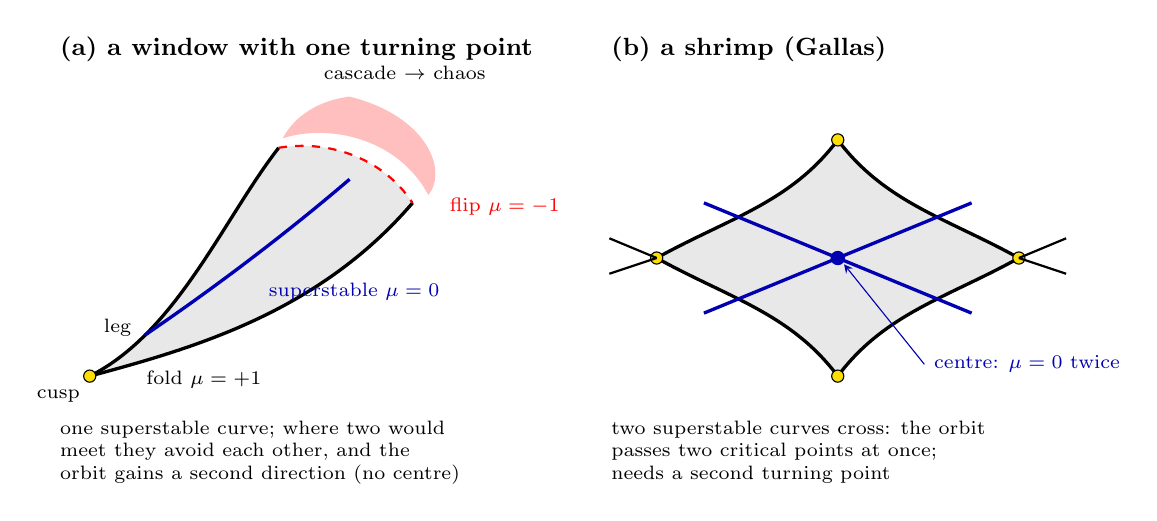
\begin{tikzpicture}[x=1cm,y=1cm,>=stealth]
  % ---------------- (a) window of a one-humped family ----------------
  \begin{scope}
    % body: region between two fold curves that meet in a cusp and run on as a thin leg
    \fill[gray!18] (0.3,0.4) .. controls (1.6,0.75) and (3.2,1.2) .. (4.4,2.6)
                    .. controls (4.0,3.2) and (3.3,3.4) .. (2.7,3.3)
                    .. controls (2.0,2.4) and (1.4,0.95) .. (0.3,0.4) -- cycle;
    \draw[very thick] (0.3,0.4) .. controls (1.6,0.75) and (3.2,1.2) .. (4.4,2.6);      % lower fold
    \draw[very thick] (0.3,0.4) .. controls (1.4,0.95) and (2.0,2.4) .. (2.7,3.3);     % upper fold
    \node[font=\scriptsize, anchor=south east] at (0.95,0.78) {leg};
    \fill[yellow!80!orange, draw=black] (0.3,0.4) circle (2.2pt);                      % cusp
    \node[anchor=north east, font=\scriptsize] at (0.3,0.35) {cusp};
    % flip curve near the far edge, then the cascade into chaos
    \fill[red!25] (2.75,3.42) .. controls (3.3,3.6) and (4.2,3.45) .. (4.6,2.7)
                   .. controls (4.85,3.0) and (4.6,3.7) .. (3.6,3.95) .. controls (3.2,3.9) and (2.9,3.7) .. (2.75,3.42) -- cycle;
    \draw[red, thick, dashed] (2.7,3.3) .. controls (3.3,3.4) and (4.0,3.2) .. (4.4,2.6);
    \node[red, font=\scriptsize, anchor=west] at (4.75,2.55) {flip $\mu=-1$};
    \node[font=\scriptsize, align=center] at (4.3,4.25) {cascade $\to$ chaos};
    % the one superstable curve (multiplier 0) through the body
    \draw[blue!70!black, very thick] (1.0,0.92) .. controls (2.0,1.6) and (2.9,2.3) .. (3.6,2.9);
    \node[blue!70!black, font=\scriptsize, anchor=north west] at (2.45,1.7) {superstable $\mu=0$};
    \node[font=\scriptsize] at (1.75,0.35) {fold $\mu=+1$};
    \node[font=\small\bfseries, anchor=west] at (-0.2,4.55) {(a) a window with one turning point};
    \node[font=\scriptsize, align=left, anchor=north west] at (-0.2,-0.05)
      {one superstable curve; where two would\\ meet they avoid each other, and the\\ orbit gains a second direction (no centre)};
  \end{scope}
  % ---------------- (b) Gallas shrimp ----------------
  \begin{scope}[xshift=7.2cm]
    \fill[gray!18] (0.3,1.9) .. controls (1.2,2.4) and (2.0,2.6) .. (2.6,3.4)
                    .. controls (3.2,2.6) and (4.0,2.4) .. (4.9,1.9)
                    .. controls (4.0,1.4) and (3.2,1.2) .. (2.6,0.4)
                    .. controls (2.0,1.2) and (1.2,1.4) .. (0.3,1.9) -- cycle;
    \draw[very thick] (0.3,1.9) .. controls (1.2,2.4) and (2.0,2.6) .. (2.6,3.4)
                    .. controls (3.2,2.6) and (4.0,2.4) .. (4.9,1.9)
                    .. controls (4.0,1.4) and (3.2,1.2) .. (2.6,0.4)
                    .. controls (2.0,1.2) and (1.2,1.4) .. (0.3,1.9);
    \foreach \p in {(0.3,1.9),(2.6,3.4),(4.9,1.9),(2.6,0.4)} {\fill[yellow!80!orange, draw=black] \p circle (2.2pt);}
    % four legs leaving the cusps
    \draw[thick] (0.3,1.9) -- (-0.3,2.15); \draw[thick] (0.3,1.9) -- (-0.3,1.7);
    \draw[thick] (4.9,1.9) -- (5.5,2.15); \draw[thick] (4.9,1.9) -- (5.5,1.7);
    % two superstable curves crossing at the centre
    \draw[blue!70!black, very thick] (0.9,1.2) -- (4.3,2.6);
    \draw[blue!70!black, very thick] (0.9,2.6) -- (4.3,1.2);
    \fill[blue!70!black] (2.6,1.9) circle (2.6pt);
    \node[blue!70!black, font=\scriptsize, anchor=west] (c) at (3.7,0.55) {centre: $\mu=0$ twice};
    \draw[->, blue!70!black] (c.west) -- (2.68,1.82);
    \node[font=\small\bfseries, anchor=west] at (-0.4,4.55) {(b) a shrimp (Gallas)};
    \node[font=\scriptsize, align=left, anchor=north west] at (-0.4,-0.05)
      {two superstable curves cross: the orbit\\ passes two critical points at once;\\ needs a second turning point};
  \end{scope}
\end{tikzpicture}
\caption{What the shrimp-like shapes are. (a) A periodic window of a two-parameter family whose reduced dynamics has
one turning point: fold curves (black; multiplier $+1$) bound the body and meet in a cusp (gold), from which the window
runs on as a thin leg; a flip curve (red, dashed; multiplier $-1$) opens a doubling cascade into chaos; one superstable
curve (blue; multiplier $0$) runs through the body. This is the anatomy we find, down to the located cusps and the
cascades. (b) A shrimp in the sense of Gallas has in addition a centre where two superstable curves of the same orbit
cross, which requires a second turning point. In the hostile period-7 body the superstable curves approach and turn
away instead, and at their closest approach the orbit's linearization has two comparable leading directions
(Figure~\ref{fig:superstable}).}
\label{fig:shrimpschematic}
\end{figure}
